%!TEX root =  main.tex
\setcounter{chapter}{11}
\setcounter{section}{2}
\setcounter{theorem}{0}
\setcounter{equation}{0}

\lectureheader{162}{Calculus II}{Calculus on parametric equations}{\textit{Thomas' Calculus} \thesection} 

\begin{theorem}
If $x$ and $y$ are given as functions of the parameter $t$, then
\begin{equation*}
\frac{\dee y}{\dee x} = \frac{\frac{\dee y}{\dee t}}{\frac{\dee x}{\dee t}}
\end{equation*}
whenever $\DS\frac{\dee x}{\dee t}\ne 0$.
\end{theorem}

\begin{remark}
Observe that if $x$ and $y$ are measuring distances in space, then $\frac{\dee y}{\dee x}$ is ``unitless," consistent with its interpretation as a slope (i.e., a direction in the $xy$-plane).
If we imagine that $t$ is measuring time, then it becomes clear why neither $\frac{\dee x}{\dee t}$ not $\frac{\dee y}{\dee t}$ can give us the slope at a spatial point on the curve: they both have the wrong units.
\end{remark}

\begin{example}
Find the tangent line to the curve
\begin{align*}
x &= \sec t,\\
y &= \tan t
\end{align*}
at the point $(\sqrt 2, 1)$, i.e., when $t=\pi/4$.
\end{example}
\ifdefined\SOLUTION
\SOLUTION{
Observe that
\begin{align*}
\frac{\dee x}{\dee t}&=\sec(t)\tan(t),\\
\frac{\dee y}{\dee t}&=\sec^2{t}, 
\end{align*}
and so
\begin{equation*}
\frac{\dee y}{\dee x}
=\frac{\frac{\dee y}{\dee t}}{\frac{\dee x}{\dee t}}
=\frac{\sec^2(t)}{\sec(t)\tan(t)}
=\sec(t)\cot(t)
=\frac{1}{\sin t}
=\csc(t).
\end{equation*}
Whence,
\begin{equation*}
\frac{\dee y}{\dee x}\Big|_{(x,y)=(\sqrt{2},1)}
=\csc(\pi/4) 
=\sqrt{2}.
\end{equation*}
Therefore, an equation for the tangent at $(\sqrt{2},1)$ is 
\begin{equation*}
y-1=\sqrt{2}(x-\sqrt{2}).
\end{equation*}
}
\fi
\newpage

\begin{example}
Compute $\DS\frac{\dee^2 y}{\dee x^2}$ as a function of $t$ is
\begin{align*}
x & = t-t^2,\\
y &= t-t^3.
\end{align*}
\end{example}
\ifdefined\SOLUTION
\SOLUTION{
First, we compute that
\begin{align*}
\frac{\dee x}{\dee t} &= 1-2t,\\
\frac{\dee y}{\dee t} &= 1-3t^2,\\
\end{align*}
and so
\begin{equation*}
\frac{\dee y}{\dee x}
=\frac{\dee y}{\dee t}\Big/\frac{\dee x}{\dee t}
=\frac{1-3t^2}{1-2t}.
\end{equation*}
Now applying the same logic with $y$ replaced by $\dee y/\dee t$, we see that
\begin{equation*}
\frac{\dee^2 y}{\dee x^2}
=\frac{\dee}{\dee x}\left( \frac{\dee y}{\dee x}\right)
=\frac{\frac{\dee}{\dee t}\left(\frac{\dee y}{\dee x}\right)}{\frac{\dee x}{\dee t}}. 
\end{equation*}
Since
\begin{align*}
\frac{\dee}{\dee t}\left( \frac{\dee y}{\dee x}\right)
&=\frac{(1-2t)(-6t)-(1-3t^2)(-2)}{(1-2t)^2} \\
&=\frac{-6t+12t^2+2-6t^2}{(1-2t)^2} \\
&=\frac{6t^2-6t+2}{(1-2t)^2}
\end{align*}
we have that
\begin{equation*}
\frac{\dee^2 y}{\dee x^2}
=\frac{6t^2-6t+2}{(1-2t)^2}\Big/(1-2t)
=\frac{6t^2-6t+2}{(1-2t)^3}.
\end{equation*}
}
\fi
\newpage

\begin{remark}\,
\begin{itemize}
\item The substitution rule (i.e., chain rule in reverse) can help us compute areas in parametric form as well.
\item If $y$ is a function of $x$ and $x$ is a function of $t$, then
\begin{equation*}
\int_{x(a)}^{x(b)}y\dee x = \int_a^b y(t)\frac{\dee x}{\dee t}\dee t.
\end{equation*}
\end{itemize}
\end{remark}

\begin{example}
Find the area enclosed by the astroid
\begin{align*}
x &= \cos^3 t,\\
y &= \sin^3 t\quad (0\le t\le 2\pi).
\end{align*}
\begin{flushright}
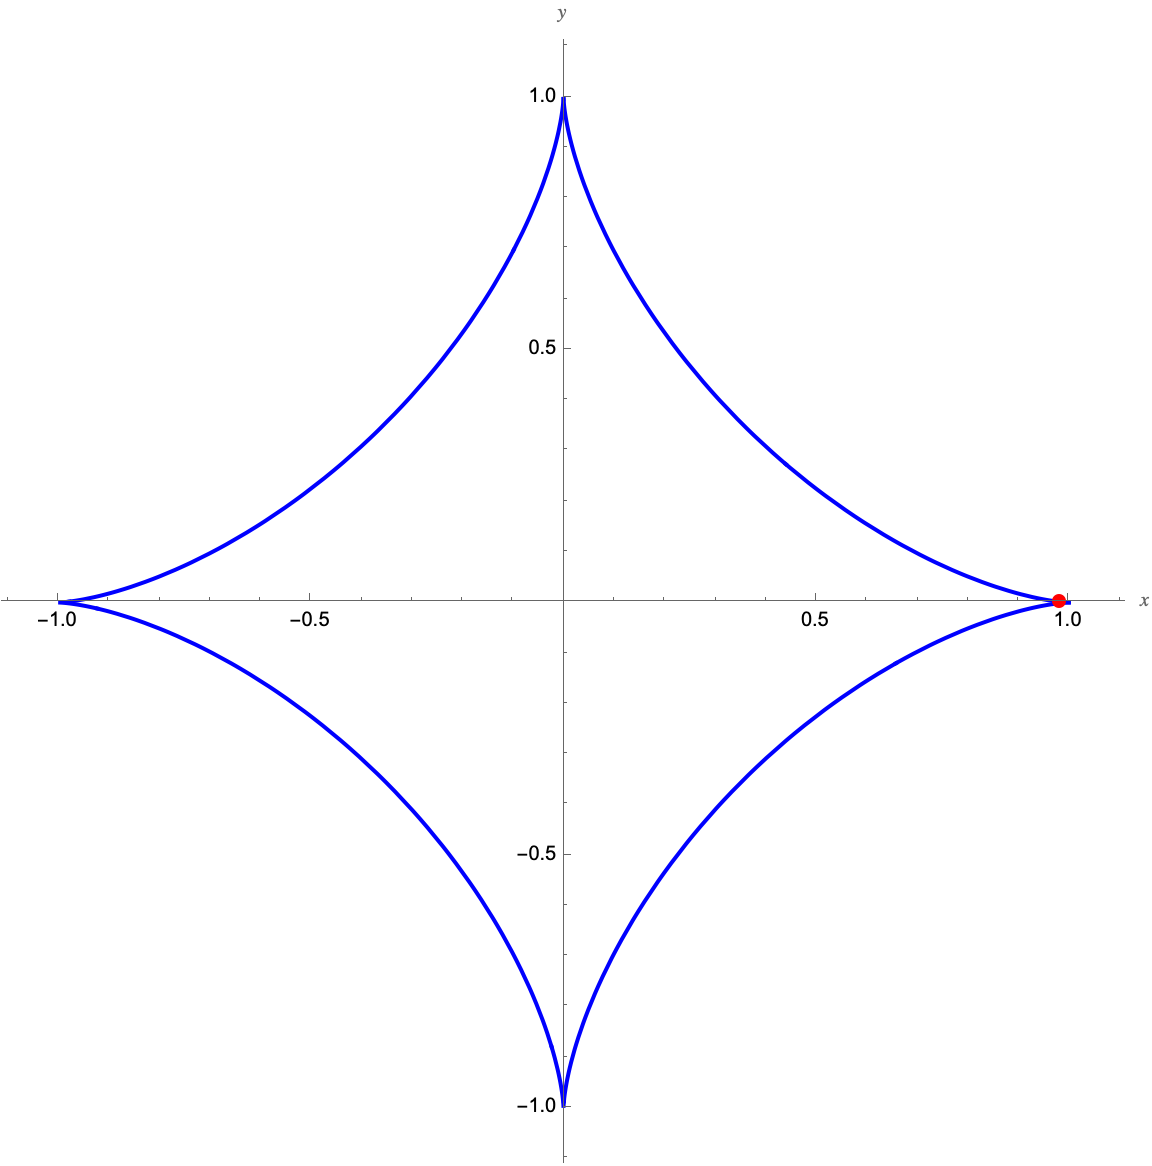
\includegraphics[width=2.5in]{img/astroid}
\end{flushright}
\end{example}
\ifdefined\SOLUTION
\SOLUTION{
By symmetry, the area of the astroid is 4 times the area of the portion that lies in the first quadrant.
Whence,
\begin{align*}
A &= 4\int_0^1 y\dee x
=4\int_{\pi/2}^0 y(t)\frac{\dee x}{\dee t}\dee t
=4\int_{\pi/2}^0\sin^3(t)\big(-3\cos^2(t)\sin(t)\big)\dee t\\ 
&=12\int_0^{\pi/2}\sin^4(t)\cos^2(t)\dee t
=12\int_0^{\pi/2}\left(\frac{1-\cos(2t)}{2}\right)^2\left(\frac{1+\cos(2t)}{2}\right)\dee t\\
&=\frac{12}{8}\int_0^{\pi/2}\left(1-\cos^2(2t)\right)(1-\cos(2t))\dee t\\
&=\frac{3}{2}\int_0^{\pi/2}\sin^2(2t)(1-\cos(2t))\dee t\\
&=\frac{3}{2}\left(\int_0^{\pi/2}\sin^2(2t)\dee t-\int_0^{\pi/2}\sin^2(2t)\cos(2t)\dee t\right)\\
&=\frac{3}{2}\left(\int_0^{\pi/2}\frac{1-\cos(4t)}{2}\dee t-\frac{1}{2}\int_0^{\pi/2}\sin^2(2t)\dee\big(\sin(2t)\big)\right)\\
&=\frac{3}{4}\left(t-\frac{1}{4}\sin(4t)-\frac{1}{3}\sin^3(2t)\right)\Bigg|_0^{\pi/2}
=\frac{3\pi}{8}.
\end{align*}
}
\else
\newpage
\fi

\begin{definition}
Given a parametric curve $C$ that is traversed exactly once as $t$ varies from $\alpha$ to $\beta$, we define the \textbf{arc length differential} by
\begin{equation*}
\dee s = \sqrt{\dee x^2 + \dee y^2},
\end{equation*}
and we define the \textbf{arc length} of $C$ by
\begin{equation*}
s = \int_C\dee s = \int_\alpha^\beta\sqrt{\left(\frac{\dee x}{\dee t}\right)^2 + \left(\frac{\dee y}{\dee t}\right)^2}\dee t
\end{equation*}
provided that the integral exists.
\end{definition}

\begin{remark}\,
\begin{itemize}
\item It is tradition to denote arc length by $s$ for the Latin \textit{spatium}.
\item The definition of $\dee s$ is based on the distance formula and is meant to signify an ``infinitesimal" distance traveled \textit{along} the curve $C$.  
\item In particular, if $C$ passes through the points $(x_{i-1}, y_{i-1})$ and $(x_i, y_i)$, then then distance $\Delta s_i$ traveled \textit{along} $C$ between these two points may be approximated by the straight line distance between the two points, i.e.,
\begin{equation*}
\Delta s_i \approx \sqrt{\Delta x_i^2 + \Delta y_i^2},
\end{equation*}
where $\Delta x_i = x_i-x_{i-1}$ and $\Delta y_i = y_i - y_{i-1}$.
\item Observe that $\dee s$ has the correct units of length attached to it.
\end{itemize}
\end{remark}
\newpage

\begin{example}
Compute the length of the astroid
\begin{align*}
x &= \cos^3 t,\\
y &= \sin^3 t\quad (0\le t\le 2\pi).
\end{align*}
\end{example}
\ifdefined\SOLUTION
\SOLUTION{
Observe that
\begin{align*}
\frac{\dee x}{\dee t}&=-3\cos^2(t)\sin(t),\\
\frac{\dee y}{\dee x}&=3\sin^2(t)\cos(t),
\end{align*}
and hence
\begin{equation*}
\begin{split}
\dee s
&=\sqrt{\left(\frac{\dee x}{\dee t}\right)^2+\left(\frac{\dee y}{\dee t}\right)^2}\dee t\\
&=\sqrt{(-3\cos^2(t)\sin(t))^2+(3\sin^2(t)\cos(t))^2}\\
&=\sqrt{\sin^2(t)\cos^2(t)(\cos^2(t) + \sin^2(t))}\dee t\\
&=\left| \sin t \cos t \right|\dee t.
\end{split}
\end{equation*}
Using symmetry to argue as before, we see that the total length of the curve is 4 times the length that lies in the first quadrant.
Therefore, the arc length
\begin{equation*}
s=\int_C \dee s 
=3\int_0^{2\pi} \left| \sin t \cos t \right|\dee t
=12\int_0^{\pi/2} \sin t\cos t \dee t 
=12\frac{\sin^2 t}{2}\Big|_0^{\pi/2} 
=6(1-0)
=6.
\end{equation*}
}
\else
\fi
\newpage



\begin{definition}
Suppose that the parametric curve $C$ is traversed exactly once as $t$ varies from $\alpha$ to $\beta$.
If $C$ is rotated about the $x$-axis to generate a surface of revolution $S$, we define the \textbf{(surface) area} $A$ of the resulting \textit{surface of revolution} by
\begin{equation*}
A = \int_C 2\pi y\dee s =2\pi \int_\alpha^\beta y(t)\sqrt{\left(\frac{\dee x}{\dee t}\right)^2 + \left(\frac{\dee y}{\dee t}\right)^2}\dee t
\end{equation*}
provided that the integral exists.
\end{definition}

\begin{remark}\,
\begin{itemize}
\item If $C$ is rotated about the $y$-axis, then 
\begin{equation*}
A = \int_C 2\pi x\dee s =2\pi \int_\alpha^\beta x(t)\sqrt{\left(\frac{\dee x}{\dee t}\right)^2 + \left(\frac{\dee y}{\dee t}\right)^2}\dee t.
\end{equation*}
\item The definition is based off the area of the \textit{frustum} of a cone.
\item Observe that, in either case, $A$ has the correct dimensionality.
\end{itemize}
\end{remark}

\newpage

\begin{example}
Calculate the area of the surface that is generated by rotating the curve $y=\sqrt{4-x^2}$ for $-1\le x\le 1$ about the $x$-axis.
\end{example}
\ifdefined\SOLUTION
\SOLUTION{
Since we are rotating about the $x$-axis we use the formula
\begin{equation*}
    A = \int_C 2\pi y\dee s.
\end{equation*}
We then choose the ``natural parametrization" 
\begin{align*}
x&=t,\\
y&=\sqrt{4-t^2}, \quad (-1 \le t \le 1)
\end{align*}
for the generating curve.
With this choice, we find that
\begin{align*}
\frac{\dee x}{\dee t}&=1,\\
\frac{\dee y}{\dee t}&=\frac{-t}{\sqrt{4-t^2}},
\end{align*}
and so
\begin{equation*}
\dee s
=\sqrt{\left(\frac{\dee x}{\dee t}\right)^2+\left(\frac{\dee y}{\dee t}\right)^2}\dee t
=\sqrt{1 + \frac{t^2}{4-t^2}}\dee t 
=\sqrt{\frac{4}{4-t^2}}\dee t 
=\frac{2\dee t}{\sqrt{4-t^2}}.
\end{equation*}
Therefore, the surface area
\begin{equation*} 
A=2\int_0^1 2\pi\sqrt{4-t^2}\frac{2}{\sqrt{4-t^2}}\dee t 
=8\pi\int_0^1\dee t 
=8\pi.
\end{equation*}
}
\else
\fi
\newpage

\begin{example}
Show that Gabriel's horn has infinite surface area despite having finite volume.
\end{example}
\ifdefined\SOLUTION
\SOLUTION{
Gabriel's horn is generated by rotating the curve $y=1/x$  around the $x$-axis for $1\le x<\infty$.  
Using the disk method, the volume of the horn
\begin{align*}
V = \int_0^{\infty}\pi\left(\frac{1}{x}\right)^2\dee x
= \pi \lim_{x\to\infty}\int_1^t \frac{\dee x}{x^2} 
= \pi\lim_{x\to\infty} \left.-\frac{1}{x}\right|_1^t 
= \pi\lim_{t\to\infty}\left(1-\frac{1}{t}\right) = \pi.
\end{align*}
To compute the surface area
\begin{equation*}
    A = \int_1^{\infty}2\pi y\dee s,
\end{equation*}
we choose the parametrization $x=t$ and $y = 1/t$ with $t\ge 1$. 
With this choice, $\frac{\dee x}{\dee t} = 1$, $\frac{\dee y}{\dee t} = -t^{-2}$, and $\dee s = \sqrt{1 + \frac{1}{t^4}}\dee t$.
Whence,
\begin{equation*}
A = 2\pi\int_1^{\infty}\frac{1}{t}\sqrt{1 + \frac{1}{t^4}}\dee t.
\end{equation*}
Now observe that
\begin{equation*}
\frac{1}{t}\sqrt{1+\frac{1}{t^4}}\ge\frac{1}{t}\sqrt{1+1} > \frac{1}{t} > 0\quad (t\ge 1),
\end{equation*}
and since 
\begin{equation*}
\int_0^{\infty}\frac{\dee t}{t} = \infty,
\end{equation*}
the direct comparison test implies that 
\begin{equation*}
A = 2\pi\int_1^{\infty}\frac{1}{t}\sqrt{1 + \frac{1}{t^4}}\dee t = \infty.
\end{equation*}
}
\fi
